% +------------------------------------------------------------------------+
% | Reference manual chapter: overlay_ref.tex (Map Overlay)
% +------------------------------------------------------------------------+
% | 
% | Package: ovl (Map Overlay)
% | 
% +------------------------------------------------------------------------+

%+----------------------------------------------------------------------------80
%| update log
%|
%| 01 April 2002 - Eti Ezra
%|    Separated from map_overlay.tex (See previous changes in change log there).
%|     
%+----------------------------------------------------------------------------80


% +========================================================================+
%   Introduction
% +========================================================================+
%\clearpage
%\section{Reference Pages for 2D Planar Maps}
%\ccRefLabel{Pm_Ref_intro}

\chapter{2D Map Overlays}
\label{chap:map_overlay_2_ref}
\ccRefLabel{Ovl_Ref_intro}
\section{Introduction}

Given two planar subdivisions $R$ and $B$, 
the overlay of $R$ and $B$, 
denoted by $O(R,B)$, is the subdivision of the plane 
induced by the edges of $R$ and $B$.
We refer to the components of $R$ as red, 
and to the components of $B$ as blue.
$R$ and $B$ are also called the {\em creators} of $O(R,B)$.
The overlay $O(R,B)$ consists of all non-empty sets $r \cap b$, 
such that $r \in R$ and $b \in B$. 
Every such non-empty set in $O(R,B)$ maintains 
pointers to the components $r \in R$ and $b \in B$ that created it.
More specifically, if a component $o \in O(R,B)$ points 
to the respective components $r \in R$ and $b \in B$, 
we say that $r$ and $b$ lie {\em above} $o$, 
alternatively, we say that $o$ lies {\em below} $r$ and $b$.
Figure~\ref{OVL_sec:overlay_example} displays an overlay 
of two given rectangles.

We can divide the problem of computing $O(R,B)$ into two subproblems:
\begin{itemize}
\item reporting all intersections between $R$ and $B$.
This subproblem is related to the red-blue curve intersection 
problem: Given a set of non-intersecting red curves and a 
set of non-intersecting blue curves in the plane, 
with a total of $N$ curves, report all $k$ intersections of 
red curves and blue curves.
In our implementation we construct the arrangement of the 
red and the blue curves by two possible algorithms:
the {\it incremental} algorithm and the {\it sweep-line} 
algorithm (See section~\ref{sec:algorithms}. 
In the implementation of the incremental algorithm 
we use the \ccStyle{Planar_Map_with_Intersections} class 
in order to represent the arrangement in construction,
and in our implementation to the sweep-line algorithm 
we simply use the \ccc{Sweep_Line_2} package.
In the latter case we use a \ccStyle{Planar_map_2} class
in order to represent the arrangement in construction.

\item updating each component $o \in O(R,B)$ to point to the 
respective components of $R$ and $B$ that created it.
This subproblem is easier than the former one,
and can be solved by a single pass on the arrangement 
constructed in the former stage.
In our implementation, we define a special \ccStyle{DCEL}
for the \ccc{Map_Overlay_2} package,
which is the data structure representing the constructed arrangement 
induced by the overlay (see Section~\ref{sec:dcel}).
In addition, we use the \ccStyle{Map Overlay Notifier} 
(see Section\ref{sec:notifier}), which is 
a newly defined class containing methods for updating the pointers 
in each component of the DCEL representing the 
constructed arrangement.
\end{itemize}

\begin{figure}[h]
    \begin{ccTexOnly}
        \centerline{
           \includegraphics{overlay_example.eps}
           }
    \end{ccTexOnly}
    \caption{Two rectangles (left) and their overlay (right). 
       We denote the subdivision induced by the first rectangle by $R$ and the second by $B$. 
       The face $f$ of the overlay is below $f_1$ and the unbounded face of $B$. 
       The halfedge $e$ of the overlay contains a halfedge pointer to $e_2$ and two face pointers 
       to $f_1$ and to $f_2$ (note that $e$ lies in the interior of $f_1$). 
       The vertex $v$ of the overlay points to $v_2$, contains a halfedge 
       pointer to $e_2$ and lies below $f_1$ and $f_2$.}
    \label{fig:overlay_example}
\end{figure}


\begin{ccTexOnly}

\section{Software Design}
The \ccc{Map_overlay_2<Subdivision,Notifier>} class 
is a data structure for maintaining 2D map overlays.
The data structure maintains the subdivision induced by overlaying 
the two creators, and the two pointers to these creators. 
The underlying combinatorial structure is determined by
(i) {\it Subdivision} which presents the subdivision type 
representing the overlay and its two creators. 
{\it Subdivision} can be either \ccStyle{Planar_Map_2} or, 
 \ccStyle{Planar_Map_With_Intersections_2}.
% or an a \ccc{Arrangement}.
Notice that the choice of a subdivision type determines the choice 
of a DCEL and a traits class (see Chapter~\ref{I1_ChapterPlanarMap}).
(ii) {\it Notifier} is the class used to update the overlay components. 
{\it Notifier} should be a model of the 
\ccc{PlanarMapWithIntersectionsChangeNotification_2} concept.

\subsection*{Example: Overlaying Two Subdivisions of Line Segments:}
The following example demonstrates a simple usage of the 
\ccc{Map_overlay_2<Subdivision,Notifier>} package.
In this example we construct two planar maps of line segments. 
Then we construct their overlay using the sweep-line algorithm, which is 
the default algorithm for the overlay construction. 
After the overlay is constructed, we write its corresponding planar map to the 
standard output stream. 

\ccIncludeExampleCode{Map_overlay_2/example1.C}
The input of the program is a text file containing two lists of segments, 
each of which represents an input subdivision.
\ccIncludeExampleCode{Map_overlay_2/example1.cin}

The output of the program looks like this:
\ccIncludeExampleCode{Map_overlay_2/example1.cout}

\section{Map Overlay Algorithms}
\label{sec:algorithms}
The input to our algorithms are two planar subdivisions, 
$R$ and $B$, having $N$ curves in total. 
The overlay of $R$ and $B$ has $O(N+k)$ vertices, 
where $k$ is the number of intersections between $R$ and $B$.
The combinatorial complexity of the overlay may be quadratic 
in the size of $R$ and $B$ in the worst case.

We devised and implemented two algorithms for constructing the 
arrangement induced by $R$ and $B$.
The first algorithm is the {\em incremental} algorithm, and is detailed in Section~\ref{sec:MapOverlayIncremental}. 
The second algorithm is a {\em sweep-line} algorithm 
for general curves, and is detailed in 
Section~\ref{sec:MapOverlaySweepLine}.

Both our algorithms construct the overlay by inserting 
the curves of $R$ and $B$ into the overlay.
In our software design, we used the {\it strategy pattern}, 
which enables users to implement their own map-overlay algorithms.
Any algorithm which constructs the arrangement representing 
the overlay, gets the notifier as a parameter. 
According to this design, the algorithm deals only with the construction, 
and when an update operation of the overlay components is undertaken, 
the algorithm invokes the notifier (see Section~\ref{sec:notifier}). 

\subsection*{The Incremental Algorithm}
\label{sec:MapOverlayIncremental}
The incremental algorithm constructs the arrangement representing 
$O(R,B)$ by inserting all curves of $R$ and $B$ one by one in a 
random order. 
The implementation of the incremental algorithm is straightforward, 
when using the \ccc{Planar_Map_With_Intersections_2} package: All we 
do is only randomly permute all the input curves in $R$ and $B$, 
and insert them one by one into a 
\ccStyle{Planar_Map_With_Intersections_2} object representing the 
overlay in construction.
Handling degenerate cases is gained directly from the usage of the 
\ccStyle{Planar_Map_With_Intersection} class.

\subsection*{The Sweep Line Algorithm}
\label{sec:MapOverlaySweepLine}
The sweep-line algorithm constructs the arrangement induced by $O(R,B)$, 
by sweeping all curves in $R$ and in $B$ simultaneously. 
In our implementation we employ the \ccc{Sweep Line} 
package~\ref{I1_ChapterSweepLine}. 
The sweep-line algorithm requires $O(N\log{N} + k\log{N})$ time,
where $N$ and $k$ are defined as before.

Our sweep-line algorithm supports not only segments but rather 
general curves, and hence, users may work on any type of curves by 
providing a suitable \ccStyle{Traits} class, and 
gain all the sweep-line functionality.
In addition, the sweep-line implementation supports degenerate cases, 
such as, vertical curves, several curves meeting in a common point, 
tangency between two different curves and overlapping curves.
In the latter case, the sweep-line implementation can report all overlaps
in a given collection of curves.
Handling degeneracies is achieved straightforwardly by using the 
\ccc{Sweep Line} package.

An important advancement, achieved by using the sweep-line algorithm, 
as shown by our experimental results,
is the ability to construct the overlay much faster.
In general, it is much faster to perform the sweep-line algorithm on
a collection of input curves in order to produce their planar map,
rather using the \ccc{Planar_map_with_intersections_2<Planar_map>} package,
due to an efficient calculation of intersections and avoiding the usage of
point-location operations when inserting curves into the subdivision 
associated with the overlay (when using the sweep-line algorithm this 
subdivision should be a \ccStyle{Planar_Map}, 
as recommended in~\ref{I1_ChapterSweepLine}).

In addition, the sweep-line implementation has been optimized in order to
save the usage of geometric predicates. 
Hence, users are most encouraged to employ the sweep-line algorithm 
and use \ccc{Planar_Map} as their subdivision. 

\subsection*{Example: Using the Incremental Algorithm:}
The following example demonstrates a usage of the 
\ccc{Map_overlay_2<Subdivision,Notifier>} package, 
while employing the incremental algorithm for constructing the overlay.
In this example we construct two planar maps of intersecting line segments. 
Then we construct their overlay using the incremental algorithm. 
After the overlay is constructed, we write to the standard output stream 
the planar map with intersections it holds. 

\ccIncludeExampleCode{Map_overlay_2/example2.C}
The input of the program is a text file containing two lists of segments, 
each of which represents an input subdivision.
\ccIncludeExampleCode{Map_overlay_2/example2.cin}

The output of the program looks like this:
\ccIncludeExampleCode{Map_overlay_2/example2.cout}

\section{Map Overlay DCEL}
\label{sec:dcel}

\begin{figure}[h]
    \begin{ccTexOnly}
        \centerline{
           \includegraphics{simple_overlay.eps}
           }
    \end{ccTexOnly}
\caption{Two segments (left) and their overlay (right). 
We denote the subdivision induced by the first segment by $R$ and the second by $B$. 
The vertex $v$ of the overlay, created by the intersection of the two input segments, 
points to $e_1$ and $e_2$.}
\label{fig:simple_overlay_example}
\end{figure}

The \ccc{Map_overlay_default_dcel<Traits,Vertex_base,Halfedge_base,Face_base>}
class is the data structure representing the DCEL of the overlay. 
We denote the above DCEL by $OD$.
The basic components of $OD$ are built 
on top of the basic components of the \ccStyle{Planar_Map} or 
the \ccStyle{Planar_Map_With_Intersections} 
(depending on the subdivision choosen in 
order to represent the overlay and its two creators).

The additional information we maintain in the components of $OD$ 
is the pointers to the components of the creators $R$ and $B$.
Namely, every component $o \in O(R,B)$ points to the 
respective components $r \in R$ and $b \in B$ that created it. 

In the following we list all the basic components of $OD$ and 
the respective information they hold:
\begin{itemize}
\item A face $f$ of $OD$ contains two pointers 
to the two faces of $R$ and $B$ above it.
\item Each halfedge $e$ of $OD$ contains one or two pointers 
to the halfedges of $R$ and $B$ that created it. 
Note that, for halfedges, we need two pointers only 
in the case of overlapping curves. 
Each halfedge $e$ also maintains two pointers to the faces of the 
creators above it. 
In some cases, such a pointer simply refers to the face on the 
side of the halfedge above $e$, and hence, maintaining the face 
pointer does not add any new information. 
However, the latter information is necessary when $e$ lies in 
the interior of a face from $R$ or $B$.
In such cases, we can not access this information through the 
halfedges of the creators. 
See Figure~\ref{fig:overlay_example} for an illustration.
%In most such cases $e$ is a hole in a face of the overlay.
\item A vertex $v$ of $OD$ can contain up to two pointers to the 
vertices of $R$ and $B$. If $v$ was created by the overlay of 
two vertices (one from $R$ and one from $B$), then it contains 
two pointers to these vertices.
If $v$ was created only by one vertex (from $R$ or from $B$), then 
it contains one pointer to that vertex. Otherwise, if $v$ was 
created by an intersection between the interior of a curve from 
$R$ and the interior of a curve from $B$, then it does not point 
to any vertex from $R$ or $B$. 
A vertex $v$ of $OD$ also contains one or two pointers 
to the halfedges of $R$ and $B$ that contain it, where relevant. 
In some cases, a pointer to the creator halfedge can be obtained by 
accessing one of the halfedges emanating from the vertex lying above 
$v$. In this case, we pick one such halfedge arbitrarily.
However, when dealing with cases in which $v$ is an intersection 
of the interiors of two edges, 
we cannot simply access this data through a vertex of the creator.
Such a case is illustrated in Figure~\ref{fig:simple_overlay_example}.
In addition, $v$ also contains pointers to the two 
faces from $R$ and $B$ that contain it. 
If $v$ lies on the boundary of creator faces meeting at $v$,
%some faces of its creators, 
we choose one such face arbitrarily.
Maintaining the latter information is necessary 
in case $v$ lies in the interior of a creator face.
See Figure~\ref{fig:overlay_example} for an illustration.
\end{itemize}


\section{Map Overlay Notifier}
\label{sec:notifier}
Updating the DCEL additional attributes is performed by the {\em Notifier} class.
We extend and override the notification functions of the basic {\em Notifier}, 
defined in the \ccc{Planar_Map_2<Dcel,Traits>} package 
(see Chapter~\ref{I1_ChapterPlanarMap}), 
in order to update the corresponding features constructed by the overlay. 

The \ccc{Map_overlay_default_notifier<Subdivision>} class 
keeps on updating the additional information in the DCEL.
It updates the pointers to the components of the creators.
The notifier class overrides only the functions \ccStyle{add_edge} 
and \ccStyle{split_edge} of the basic notifier defined for \ccStyle{Planar_Map}.
In our implementation these functions update 
the pointers of the halfedges and the vertices in the DCEL 
presenting the overlay, see Chapter~\ref{I1_ChapterPlanarMap} for details.
In order to update the pointers of a face, we define a new function in our 
notifier, which we call \ccStyle{update_all_faces}. 
This function traverses all components in the overlay in a DFS manner and 
updates their corresponding face pointers. 
This function is invoked once we have terminated 
inserting into the overlay all the curves in $R$ and $B$.
We did not use the \ccStyle{split_face} function in order to update a 
face pointers, since it is invoked each time a cycle in the DCEL 
is closed and degrade performance. 

\section{Boolean Operations:}
A straightforward usage of the \ccc{Map_overlay_2<Subsection,Notifier>} 
utilities, is performing boolean operations on planar subdivisions in general, 
and specifically on polygons.

An object of the \ccc{Boolean_operations_2<Map_Overlay>} class is initialized with 
two input subdivisions. In the initialization step, it constructs the overlay 
of the two input subdivisions. By constructing the overlay, all boolean operations, 
on the two input subdivisions, can be easily provided.
The  \ccc{Boolean_operations_2<Map_Overlay>} class provides methods for 
performing an intersection, union, symmetric difference and difference on the two 
input subdivisions. 
The output of such operations are all resulting vertices, halfedges and faces.

\paragraph{DCEL}
\ccRefLabel{Bops_dcel}
When performing boolean operations, the overlay of the two input subdivisions is 
constructed. Hence, naturally, users may define the input subdivisions DCEL as the 
\ccc{Map_overlay_2<Subdivision,Notifier>} DCEL. 
However, an extra functionality is required: We may be interested 
to define our boolean operations only on {\it some} features of the input subdivisions.
For instance, we would like to ignore the unbounded faces of the input subdivisions.
In order to achieve this functionality, we define a DCEL for the 
\ccc{Boolean_operations_2<Map_Overlay>} class. 
The \ccc{Boolean_operations_2<Map_Overlay>} DCEL is very similar to 
the \ccc{Map_overlay_2<Subdivision,Notifier>} DCEL.
As a matter of fact, the basic components 
of the \ccc{Boolean_operations_2<Map_Overlay>} DCEL are 
derived from those of the \ccc{Map_overlay_2<Subdivision,Notifier>} DCEL, 
and in addition they contain a boolean flag indicating, 
whether a component (vertex, halfedge or face) is ignored 
when performing boolean operations.

\subsection*{Example: Performing Boolean Operations on Two Planar Maps of Line Segments:}
The following example demonstrates a simple usage of the \ccStyle{Boolean_Operations} class.
In this example we construct two planar maps of line segments. 
Then we construct a \ccStyle{Boolean_Operations} object corresponds 
having these two subsections as input. 
After this object is constructed, we perform an intersection on the two subsections. 
In this example, we are interested only in the halfedges in the intersection.
Finally, we write all resulting halfedges to the standard output stream. 

\ccIncludeExampleCode{Boolean_operations_2/example1.C}
The input of the program is a text file containing two lists of segments, 
each of which represents an input subdivision.
\ccIncludeExampleCode{Boolean_operations_2/example1.cin}

The output of the program looks like this:
\ccIncludeExampleCode{Boolean_operations_2/example1.cout}


\subsection*{Polygons Bops:}
One of the most natural usage of 
the \ccc{Map_overlay_2<Subsection,Notifier>} utilities, 
is performing boolean operations on polygons.

The above utility is a straightforward usage of the 
\ccc{Boolean_operations_2<Map_Overlay>} 
class. Hence, every operation obtained from the functions 
for boolean operations on polygons can be achieved by 
directly using the \ccc{Boolean_operations_2<Map_Overlay>} 
class. 

The goal of providing these functions, is to 
provide a simple interface for users who are 
interested only in boolean operations on 
polygons, rather than boolean operations 
on planar subdivisions of general curves.

In our interface, we provide four function objects 
for all kinds of boolean operations on polygons,
namely, for intersection, union, difference, and 
symmetric difference.
See Sections~\ref{OVL_sec:polygon_difference},
~\ref{OVL_sec:polygon_intersection},~\ref{OVL_sec:polygon_union} 
and~\ref{OVL_sec:polygon_symmetric_difference}. 

\paragraph{Traits Class}
\ccRefLabel{Polygons_bops_traits_2}
When performing boolean operations on polygons, 
we mostly use the boolean operations defined in 
\ccc{Boolean_operations_2<Map_Overlay>}.
However, we have to translate the result obtained from the 
\ccc{Boolean_operations_2<Map_Overlay>} methods to a list 
of points, a list of curves, and a list of polygons.
The two first lists can be achieved in a quite easily,
where the last one, namely the list of the polygons,
is more difficult to be translated. This is becuase 
in most cases the faces in the output obtained from the 
\ccc{Boolean_operations_2<Map_Overlay>} methods may contain holes,
where the resulting polygons must be simple.
Hence, we decompose each face containing holes to a list 
of simple polygons. The decomposition is performed by shooting 
two vertical rays downwrads and upwdards from the leftmost 
and from the rightmost vertices of each hole. 
For this purpuse we need a Traits class, containing a method 
which performs the ray shooting. 

\subsection*{Example: Performing Boolean Operations on Two Polygons:}
The following example demonstrates a simple usage of the 
\ccStyle{Polygons_union_2<Bops_traits>} class.
In this example we compute the union of two polygons.
The output is given in three list, each of which
representing all points, curves and polygons in the union.
Finally, we write all resulting polygons to the standard output stream. 

\ccIncludeExampleCode{Polygons_bops/example1.C}

The input of the program is a text file containing two lists of segments, 
the first represents a rectangle and the latter a triangle.
\ccIncludeExampleCode{Polygons_bops/example1.cin}

The output of the program looks like this:
\ccIncludeExampleCode{Polygons_bops/example1.cout}

\end{ccTexOnly}    







